%=========================================================================

%- potreba mit 10-20 vysazenych stran / 20-40 normostran
%- na jednu plne potistenou stranu se vleze 1,65 (s nadpisem chapter) nebo 2,36 (bez nadpisu) normostran

% Setting the depth of sections numbering
\setcounter{secnumdepth}{2}
% Setting the depth of sections to appear in the table of contents.
\addtocontents{toc}{\protect\setcounter{tocdepth}{1}}


%=========================================================================
%=========================================================================
\chapter{Introduction}
% 1 - 2 ns

- napad: rozdelit uvod do pokapitol (podle https://uu.diva-portal.org/smash/get/diva2:648760/FULLTEXT01.pdf):
	- background
	- related work
	- problem formulation
	- system overview
	- thesis organization

- Slouží k zasazení řešené problematiky do širšího kontextu
- o optickych dalkomerech
- vyhody systemu (pasivni radar)
- vyuziti

- v podobě stručného obsahu jednotlivých kapitol definuje strukturu písemné práce.


-- dalsi kapitoly --

 formulaci cíle práce, charakteristiku současného stavu
 řešené problematiky a teoretická a odborná východiska řešených problémů.

 

%=========================================================================
%=========================================================================
\chapter{Related work}
% 1 - 2 ns

- srovnani s ji existujicimi aktivnimi (pasivnimi) radary

%=========================================================================
%=========================================================================
\chapter{System overview} \label{txt:system_overview}
% 2 - 4 ns

- koncept systemu (rozlozeni jednotek, pouzity hardware, propojeni, ...)
- zmineni zakladniho knceptu behu celeho systemu od detekce cile az po jeho lokalizaci
- zminit zakladnich problematiky celeho systemu: zastaniceni, rektifikace, detekce, tracking, vyber jednotek pro sledovani, najezd po opticke ose, predani cile, triangulace, ...
- moznost rizeni jednotky pomoci joystiku/klavesnice
- zminit problematiku zastaniceni a rektifikace a odkaz na prislusnou kapitolu
- zminit pouziti ROS konvence co se tyka souradnych systemu

%=========================================================================
%=========================================================================
\chapter{Camera unit} \label{txt:camera_unit}
% 2 - 4 ns

- z ceho sestava camera unit (zminit manipulator i kameru)
- návrh kinematického řetězce modelu manipulátoru
- ukazat 2D diagramy, 3D model z rvizu/gazeba
- fotka
- schema, kde bude ukazano, co je azimuthal a elevation axis

- PTU Flir
	- HW/SW limity pohybu
	- krokove motory
	- proble proklouznuti kroku
	- configuration space \cite{Russell:2009:AIM:1671238}

- nejake info o kamere


%=========================================================================
%=========================================================================
\chapter{Sensitivity analysis} \label{txt:sensitivity_analysis}
The precision of the system can be defined in the means of the frame-by-frame Euclidean distance between the estimated location and the real (ground truth) location of the given target. The precision is impacted by multiple independent factors, thus it is essential to perform the sensitivity analysis in order to discover and prospectively alleviate the most prominent contributors of the overall error. 

- vysvetleni typu chyb:
	- system error (systemova chyba)
		- nesoulad modelu CU s realnou konstrukci
		- nespravne mereni heading
		- detekce a tracking ?
	- uncertainty of the input of the system
		- GPS mereni
		- data inklinometru
	
- vysvetlit, ze se budeme snazit potlacit jen nektere chyby (neresime treba nepresnost mezi modelem a realnou CU z hledsiak translaci mezi klouby)

- rozdeleni na chybu rotace a translace
	- nepresnost v rotaci je daleko zavaznejsi, nez nepresnost v translaci
	- priklad a obrazek vlivu nepresnosti o x mrad na lokalizaci cile ve vzdalenosti y m/km

- zdroj chyb:
	- detekce
	- tracking
	- GPS pozice
	- natoceni vuci severu
	- rozliseni PTU
	- model PTU - translace mezi klouby
	- model PTU - rotace mezi klouby
	- uchyceni kamery
		- rotace podle opticke osy
		- rotace podle osy azimutu
		- rotace podle osy elevace
		
%- vysvetleni input a output systemu a pojmu sensitivity analysis (http://samples.sainsburysebooks.co.uk/9780470725177_sample_389211.pdf)

%=========================================================================
%=========================================================================
\chapter{Stationing and rectification}
% 2,5 - 3,5 ns

As explained in section \ref{txt:sensitivity_analysis} the precision of the whole system is dependent on on the uncertainty of the system input as well as on the imprecision of the camera unit construction. The process of stationing aims to alleviate the uncertainty of the system input while the main purpose of the rectification is to reduce the difference between the real camera unit and its model.

%-------------------------------------------------------------------------
%-------------------------------------------------------------------------
\section{Stationing}

Since the stationing is considered to be already working subsystem of the whole project (and thus is not dealt with within the scope of this work) only the main principle will be briefly described. The stationing is composed of two parts: finding the geographical north and finding the relative azimuthal and elevation angles between each pair of camera units.

%.........................................................................
%.........................................................................
\subsection{Geographical north} \label{txt:geographical_north}

Though it is common practice to estimate the heading\footnote{Heading is the term used to describe the angle between the torso of the human body and the geographical north \cite{Henriksson648760}} using the magnetometer, this device is unsuitable for this project since the accuracy of the concurrent professional class magnetometers is insufficient (see Section \ref{txt:sensitivity_analysis}). For instance the accuracy of the magnetometers meant for compassing applications produced by Honeywell, the multinational company focusing on aerospace systems, range from hundreds to thousands of milliradians \cite{Honeywell:compassing_catalog}.

In order to find the orientation of each camera unit placed in the outdoor environment, distinctive landmarks (created either by human or nature) with known geographical positions are used. For each such a landmark the manipulator is rotated so that the optical axis of the camera would intersect that landmark and both the azimuth and elevation value is registered. Using triangulation the geographical position of the camera unit is derived. 

Different possible approach takes advantage of the celestial objects, such as the moon, sun or stars for which the current geographical position is known as well. Nevertheless this approach can only be used between the sunset and the dawn.

%.........................................................................
%.........................................................................
\subsection{Relative azimuth and elevation}

To further reduce the impact of the uncertainty of the system input produced by the GPS (see Section \ref{txt:sensitivity_analysis}) and the system error given by the imprecision of the heading estimation (see Section \ref{txt:geographical_north}) it is convenient to find the relative position of each camera unit with regards to the rest of the camera units.

The information about the geographical position of all camera units as obtained from the GPS sensors is distributed across the whole system. Each pair of camera units then automatically performs the following:

\begin{enumerate}
	\item Set the azimuth and elevation of the manipulator so that the optical axis of the camera would intersect the expected location of the LED target of the other camera unit.
	\item Using the visual clue adjust the azimuth and elevation so that the optical axis of the camera would intersect the center of the LED target of the other unit (see Figure \ref{fig:stationing_aiming}).
	\item Save the current azimuth and elevation values of both camera units and use those values to update the model of the system.
\end{enumerate}

%% Stationing process of one pair of the camera units
\begin{figure}[htb]
	\centering
	\includegraphics[width=14cm]{fig/stationing_aiming.png}
	\caption{The schema of stationing process where two camera units attempt to align the optical axes of their cameras so that they would intersect the LED target of the other unit.}
	\label{fig:stationing_aiming}
\end{figure}


%.........................................................................
%.........................................................................
\subsection{Horizontality}
Since the camera unit is expected to be placed in an unknown outdoor terrain, it will never stand on an ideally horizontal surface. Thus it is necessary to either ensure that the unevenness of the surface is compensated by the suitable setting of the camera unit's stand or both the side tilt and front tilt angles of the stand must be estimated and integrated to the model of the given camera unit. For these purposes the inclinometer attached to the base plane of the camera unit (see Section \ref{txt:camera_unit}) is used.


%-------------------------------------------------------------------------
%-------------------------------------------------------------------------
\section{Rectification}

The process of rectification serves the purpose of reducing the system error caused by the imprecise attachment of the camera to the manipulator. The model of the camera unit assumes that the camera is precisely attached to the manipulator so that the camera image sensor is positioned perpendicular to the azimuthal axis and the rows of the image sensor are parallel to the elevation axis (i.e. the camera is not rotated along the optical axis).

Regarding these requirements the rectification consists of three parts: rotation along the optical axis, rotation along the azimuthal axis, finding the default elevation angle.


%.........................................................................
%.........................................................................
\subsection{Rotation along the optical axis}

A custom made metal mount is attached to the bottom side of the camera. The mount is then attached to the manipulator using two opposing round tenons enabling for the rotation of the mount (together with camera) along the axis parallel to the optical axis of the camera (see Figure \ref{fig:rect_model_front_view}).

%% The front view of the model of the camera unit
\begin{figure}[htb]
	\centering
	\includegraphics[width=13cm]{fig/rect_model_front_view.png}
	\caption{Front view of the top part of the camera unit. The red arrow shows the possible rotation of the camera along the axis parallel to the optical axis.}
	\label{fig:rect_model_front_view}
\end{figure}

In this part the rectification target with three parallel horizontal black lines is used. Each line has different width so that the operator can select the most suitable one (given the distance of the target, ambient lighting conditions, etc.) As the first step a surveying automatic level is used to rotate the target so that the black lines become horizontal. Then the camera is pointed approximately to the center of the target. The camera image stream is blended with the same stream mirrored across the vertical axis. The operator then manually rotates the camera so that the black lines in this blended image stream appear visually aligned (see Figure \ref{fig:rect_mirrored_stream}). Once set, the mount with the camera is fixed to the manipulator using two set screws.

%% Rectification of the rows of the camera image sensor - original stream blended with the mirrored stream
\begin{figure}[htb]
	\centering
	\includegraphics[width=13cm]{fig/rect_mirrored_stream.png}
	\caption{A blended image stream from the camera before (left) and after (right) rotating the camera along the optical axis to the correct position.}
	\label{fig:rect_mirrored_stream}
\end{figure}

%.........................................................................
%.........................................................................
\subsection{Rotation along the azimuthal axis}

The mount can still rotate along the axis parallel to the azimuthal axis (see Figure \ref{fig:rect_model_top_view}). It is necessary to ensure that the optical axis of the camera is perpendicular to the elevation axis. 

%% The top view of the model of the camera unit
\begin{figure}[htb]
	\centering
	\includegraphics[width=13cm]{fig/rect_model_top_view.png}
	\caption{Top view of the top part of the camera unit. The red arrow shows the possible rotation of the camera along the axis parallel to the azimuthal axis.}
	\label{fig:rect_model_top_view}
\end{figure}

The same target from the first part of the rectification is used, but two black crosses are added to the selected horizontal black line. The distance $d_{ao}\ m$ between two crosses equals to the distance between the azimuthal and optical axis (which is known from the engineering design, see Figure \ref{fig:rect_azi_axis}). 

%% Photograph of the camera unit with the telescope mounted on the top
%% Screenshot of the digital crosshair and the offset
\begin{figure}[htb]
	\centering
	\begin{minipage}{.42\textwidth}
		\centering
		\includegraphics[width=.99\linewidth]{fig/rect_telescope.png}
		\captionof{figure}{A telescope mounted on top of the manipulator. A person looking through a telescope sees a crosshair - a tip of a triangle.}
		\label{fig:rect_telescope}
	\end{minipage}
	\hfill
	\begin{minipage}{.54\textwidth}
		\centering
		\includegraphics[width=.99\linewidth]{fig/rect_azi_axis.png}
		\captionof{figure}{Rectification target with the pairs of black crosses. The two crosses in a pair are $d_{ao}\ m$ appart. A digital corsshair is displayed in order to find the horizontal offset $d_{h}$.}
		\label{fig:rect_azi_axis}
	\end{minipage}
\end{figure}

A military optical monocular telescope (see Figure \ref{fig:rect_telescope}) is mounted on top of the manipulator. The optical axis of the telescope intersects the azimuthal axis, it is perpendicular to it and it intersects the left cross of a given pair on the rectification target. The camera is rotated so that its optical axis (represented by the digital crosshair) intersects the right cross on the target and then is fixed using set screws. As the screws are tightened the camera is unintentionally rotated a bit again which causes the visual offset between the crosshair and the cross on the target. The offset expressed in pixels is recorded and transformed to the default angle $\beta$ expressed in milliradians (see Figure) of rotation along Z-axis of the joint \texttt{camera} in the camera unit model (see Section \ref{txt:camera_unit}):

\begin{equation*}
\begin{aligned}
\beta &= \arccos\frac{focal\_length}{offset}, \\
offset &= pixel\_offset * pixel\_size
\end{aligned}
\end{equation*}

%% Geometry schema showing how to calculate angle beta - pixel offset
\begin{figure}[htb]
	\centering
	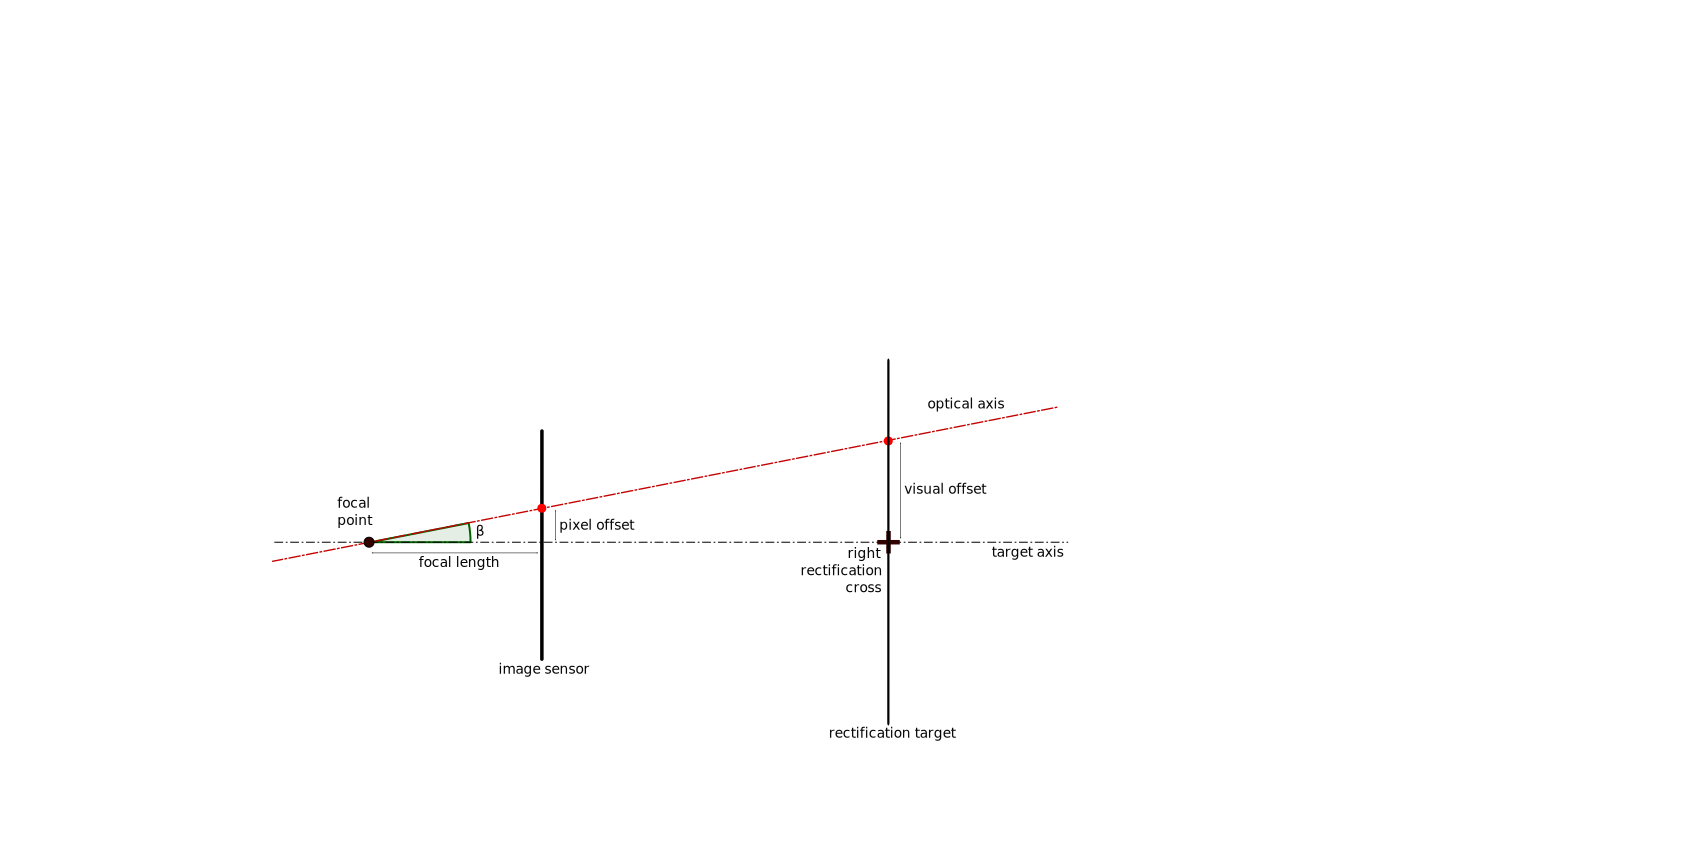
\includegraphics[width=13cm]{fig/rect_pixel_offset.pdf}
	\caption{The top view schema of a rectification target being projected to the image sensor of the camera. The value of the angle $\beta$ is one of the output of the rectification process.}
	\label{fig:rect_pixel_offset}
\end{figure}

%.........................................................................
%.........................................................................
\subsection{Finding the default elevation angle}

Given the application of the system the camera is expected to mainly observe the sky. Considering the limited elevation range of the manipulator \texttt{Flir PTU D46-70} (see Section \ref{txt:camera_unit}), the camera must be mounted to the manipulator with the default elevation angle approximately $-60^{\circ}$. However, after fixing the camera it is necessary to find default elevation angle precisely. 

For this purpose a pair of rectification targets, which consist of vertical black and white lines representing the marks of a ruler. The targets are positioned in a row with the distance of a few meters so that the front target would overlap approximately half of the rare target when observed from the camera. Both targets must be rotated so that the lines become horizontal, then the operator manually adjusts the elevation of the manipulator so that the digital crosshair would intersect the same mark on both targets where the two marks form a straight line (see figure \ref{fig:rect_default_elevation_angle}). Once found the current elevation angle is recorded and integrated to the model of the camera unit as an angle of rotation along the Y-axis of the joint \texttt{camera} (see Section \ref{txt:camera_unit}).

%% The rectification target for finding the default elevation angle.
\begin{figure}[htb]
	\centering
	\includegraphics[width=13cm]{fig/rect_default_elevation_angle.png}
	\caption{Front target of a pair of the rectification targets used to find a default elevation angle (left). A screenshot from the image stream of the camera with the crosshair focused on a row where the marks of the rulers align (right).}
	\label{fig:rect_default_elevation_angle}
\end{figure}


%=========================================================================
%=========================================================================
\chapter{Detection and tracking} \label{txt:detection_and_tracking}
% 4,5 - 9 ns

- === DETEKCE VZDALENYCH OBJEKTU V OBRAZE ===
- === SLEDOVANI OBJEKTU VE VICEKAMEROVYCH SYSTEMECH ===
- === ALGORITMY VHODNE PRO RESENI ULOHY ===

- TLD
- moznost sdileni info o appearance modelu mezi CUs


%=========================================================================
%=========================================================================
\chapter{Cooperation among camera units}
% 1 - 4 ns

- vyber druhe jednotky pro trackovani cile
- najezd po opticke ose
- predani cile


%=========================================================================
%=========================================================================
\chapter{Target localization}
% 2,5 - 6 ns

- triangulace
- === LOKALIZACE OBJEKTU VE VICEKAMEROVYCH SYSTEMECH ===
- === ALGORITMY VHODNE PRO RESENI ULOHY ===

== (obrazek z rvizu (protnuti primek) ==



%=========================================================================
%=========================================================================
\chapter{Implementation}
% 2 - 4 ns

The whole system is built on the robotic framework Robot Operating System (for details see Section \ref{txt:robot_operating_system}). Since the ROS defines multiple conventions, restrictions and best practices the whole system design including the selection of a programing language, a programing and a communication paradigm, a target platform and a tool for physical simulations is impacted by the possibilities of this framework.

As of writing this text a current state of the implementation mainly builds on the virtual environment provided by the physical simulator Gazebo (see Section \ref{txt:application_of_gazebo}). When confronted with the overview of all subsystems making up the whole system presented in Section \ref{txt:system_overview} so far the following parts are already designed, implemented and/or integrated:

\begin{itemize}
\item manual control of the manipulator using peripheral devices
\item manual selection of a target and distribution of its appearance to all CUs
\item integration and utilization of a OpenTLD tracker
\item triangulation of a 3D positions of a target within global frame
\item integration of all subsystems
\end{itemize}

Furthermore a few additional tools were utilized and/or implemented as the necessary building blocks allowing for further development and testing:

\begin{itemize}
\item a functional model of a whole system in Gazebo environment
\item a standalone application for rectification
\end{itemize}


%-------------------------------------------------------------------------
%-------------------------------------------------------------------------
\section{Robot Operating System} \label{txt:robot_operating_system}

Despite its name the ROS\footnote{The official website of ROS: \url{http://www.ros.org}} is not an operating system but rather a collection of open source libraries, tools and conventions which serve the purpose of a middlewear running alongside a real operating system, however it provides the programmer with the hardware abstraction,  low-level device control, implementation of commonly-used functionality,
message-passing between processes, and package management \cite{O'Kane201310}.

Since the original motivation for developing ROS was to support the collaboration among the experts in the field of robotics in the means of a common software platform \cite{ROS-an-open-source-Robot-Operating-System}, a huge developer community has formed around ROS which resulted in wide-scale penetration of this framework as well as the support for a huge range of hardware devices.

%.........................................................................
%.........................................................................
\subsection{Application of ROS}

The OLS is designed to become a relatively complex system, thus it exhibits non-trivial implementation requirements such as a need to distribute the computation among multiple computers, the real time performance, integration with physical simulator, etc. Since ROS is a mature framework satisfying the most of theses requirements (see Table \ref{tab:ols_requirements_ros_features}), it was chosen as a main implementation platform.


{\renewcommand{\arraystretch}{1.5}
\begin{table}[htbp]
	\centering
	\caption{The table lists the most important requirements of the OLS and describes how the ROS framework addresses them.}
	\begin{tabularx}{0.99\textwidth}{XX}
		\toprule
		\textbf{OLS requirements} & \textbf{ROS features} \\
		\midrule
		native support for hardware such as Prosilica camera, manipulator Flir PTU D46-70, joystick, keyboard & nodes implementing image capture from Prosilica cameras, capturing events from keyboards and joysticks \\
		modularity and reusability of source code & each subsystem is represented by a separate process (node), straightforward reusability \\
		distribution of computation among multiple computers & provides abstraction layer for distributing nodes across devices \\
		simple data exchange among subsystems & the publisher subscriber paradigm \cite{O'Kane201310}, support for custom message formats \\
		real time performance & C++ implementation \\
		modelling and simulating the robot & custom language \texttt{URDF}\footnotemark ~for robot modeling, integration with Gazebo \\
		specifying a kinematic chain, heavy 3D transformation computation & native support for computing transformation between frames using package \texttt{tf} \\
		complex visualization, debugging & a visualization tool \texttt{rviz}\footnotemark ~for visualizing frames, transformations, robot models, image streams etc. \\
		physical simulation & integration with Gazebo \\
		\bottomrule
	\end{tabularx}
	\label{tab:ols_requirements_ros_features}
\end{table}}

\footnotetext{Modeling language \texttt{URDF}: \url{http://wiki.ros.org/urdf}}
\footnotetext{Vsisualization tool \texttt{rviz}: \url{http://wiki.ros.org/rviz}}

%.........................................................................
%.........................................................................
\subsection{Standard ROS packages}

ROS provides a wide range of standard packages for interaction with various hardware devices. The implementation of OLS utilizes following packages:

\begin{description}
	\item[avt\_vimba\_camera\footnote{Package avt\_vimba\_camera: \url{http://wiki.ros.org/avt_vimba_camera}}] \hfill \\
	This package wraps the Vimba GigE SDK provided by Allied Vision Technologies, the manufacturer of the Prosilica series cameras, and allows the programmer to subscribe to the topic \texttt{camera\textbackslash image\_raw} and easily access the image stream.
	
	\item[keyboard\footnote{Package keyboard: \url{http://wiki.ros.org/keyboard}}] \hfill \\
	The package process the keyboard events and expose them via \texttt{keydown} and \texttt{keyup} topics.
	
	\item[joy\footnote{Package joy: \url{http://wiki.ros.org/joy}}] \hfill \\
	This package process the events from a joystick and/or gamepad and expose them via \texttt{joy} topic.
	
\end{description}
	

%-------------------------------------------------------------------------
%-------------------------------------------------------------------------
\section{System architecture}

Given the modular concept of the ROS it is most convenient to divide the whole system into autonomous subsystems represented by separate ROS packages. From the perspective of OLS this division of computation work among packages should loosely correspond to the hardware units used.

%.........................................................................
%.........................................................................
\subsection{Hardware}

Considering the big picture of the system, OLS consists of four camera stations, a hardware devices necessary for network communication and the peripherals for manual control. There are two types of camera stations, a tracking station and an overview station (see Section \ref{txt:system_overview}). All stations communicate with each other vie Ethernet switch. The peripherals allowing the operator to manually control the system are connected to the overview station (see Figure \ref{fig:hw_ols}).

%% The big picture diagram of the hardware components of the OLS
\begin{figure}[htb]
	\centering
	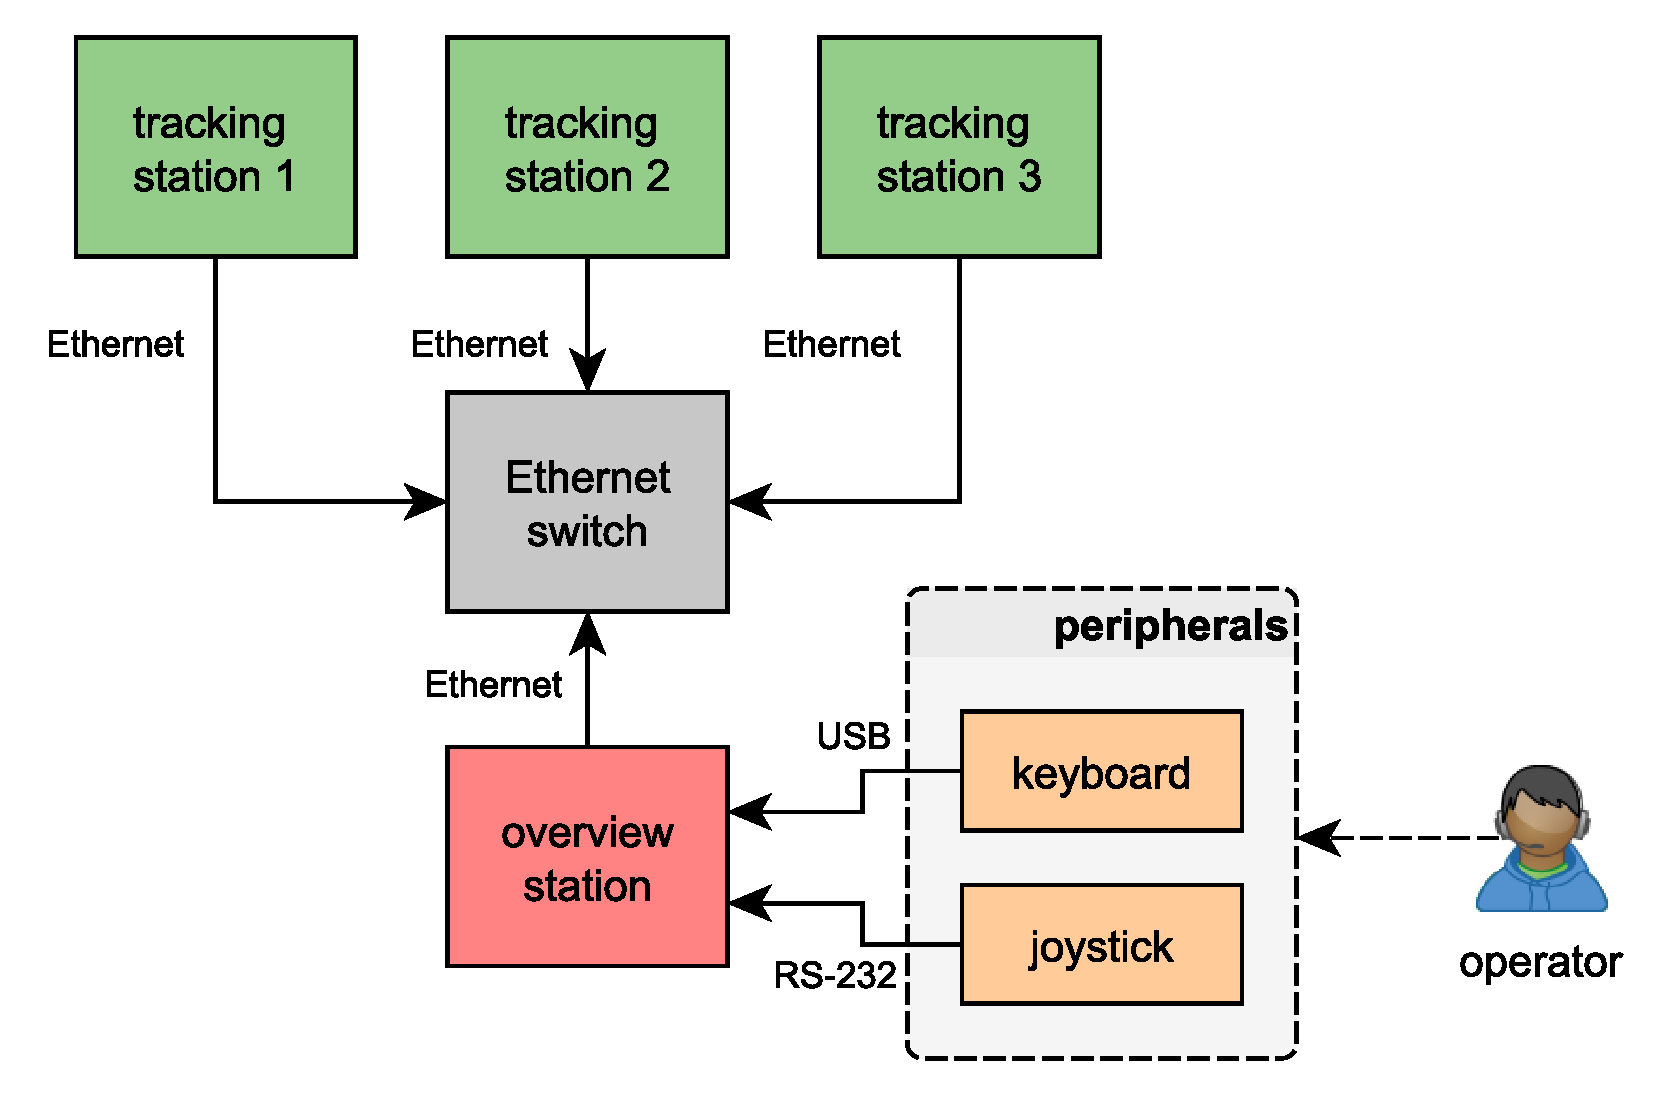
\includegraphics[width=10cm]{fig/hw_ols.pdf}
	\caption{The big picture diagram of the main components of the OLS.}
	\label{fig:hw_ols}
\end{figure}

A camera station itself consists of a camera unit (see Section \ref{txt:camera_unit}) and a computer running the OLS software. The camera unit is controlled by the controller \texttt{STM32F4007} which communicates with the manipulator \texttt{Flir PTU D46-70}, a GPS module and a zoom lense. The camera \texttt{Prosilica GT 1290C} is connected directly to a computer running OLS system (for more details see Figure \ref{fig:hw_camera_unit}).

%% The diagram of the hardware components of the camera unit
\begin{figure}[htb]
	\centering
	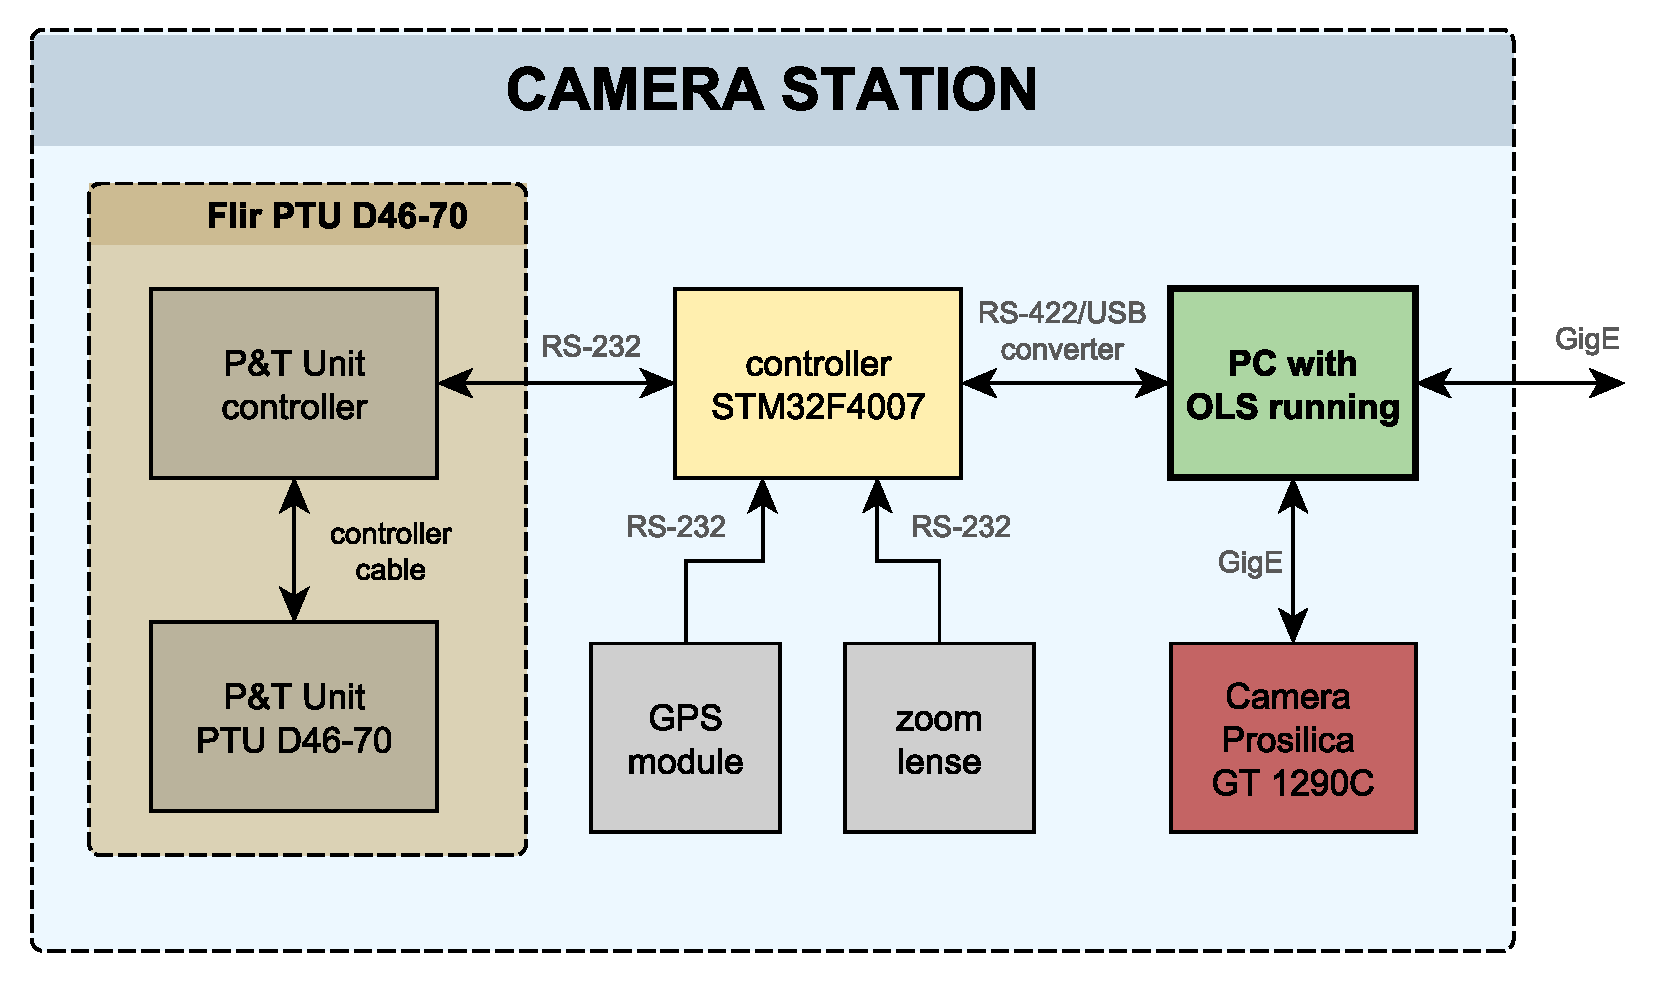
\includegraphics[width=10cm]{fig/hw_camera_unit.pdf}
	\caption{The diagram of the hardware components of the camera unit depicting both the hardware devices and the communication standards.}
	\label{fig:hw_camera_unit}
\end{figure}



%.........................................................................
%.........................................................................
\subsection{Software}

The system is divided into multiple ROS nodes (processes running in the operating system) with the aim to loosely resemble the hardware components. Five namespaces are used, one \texttt{master} namespace and four \texttt{camera\_unit\_N} namespaces, where $N \in \{0, 1, 2, 3\}$ identifies a unique camera unit. The overview of the system architecture from the perspective of the ROS namespaces, nodes, messages and services is depicted on Figure \ref{fig:sw_ols}.

%% The diagram of the software components - ROS nodes - and ROS topics.
\begin{figure}[htb]
	\centering
	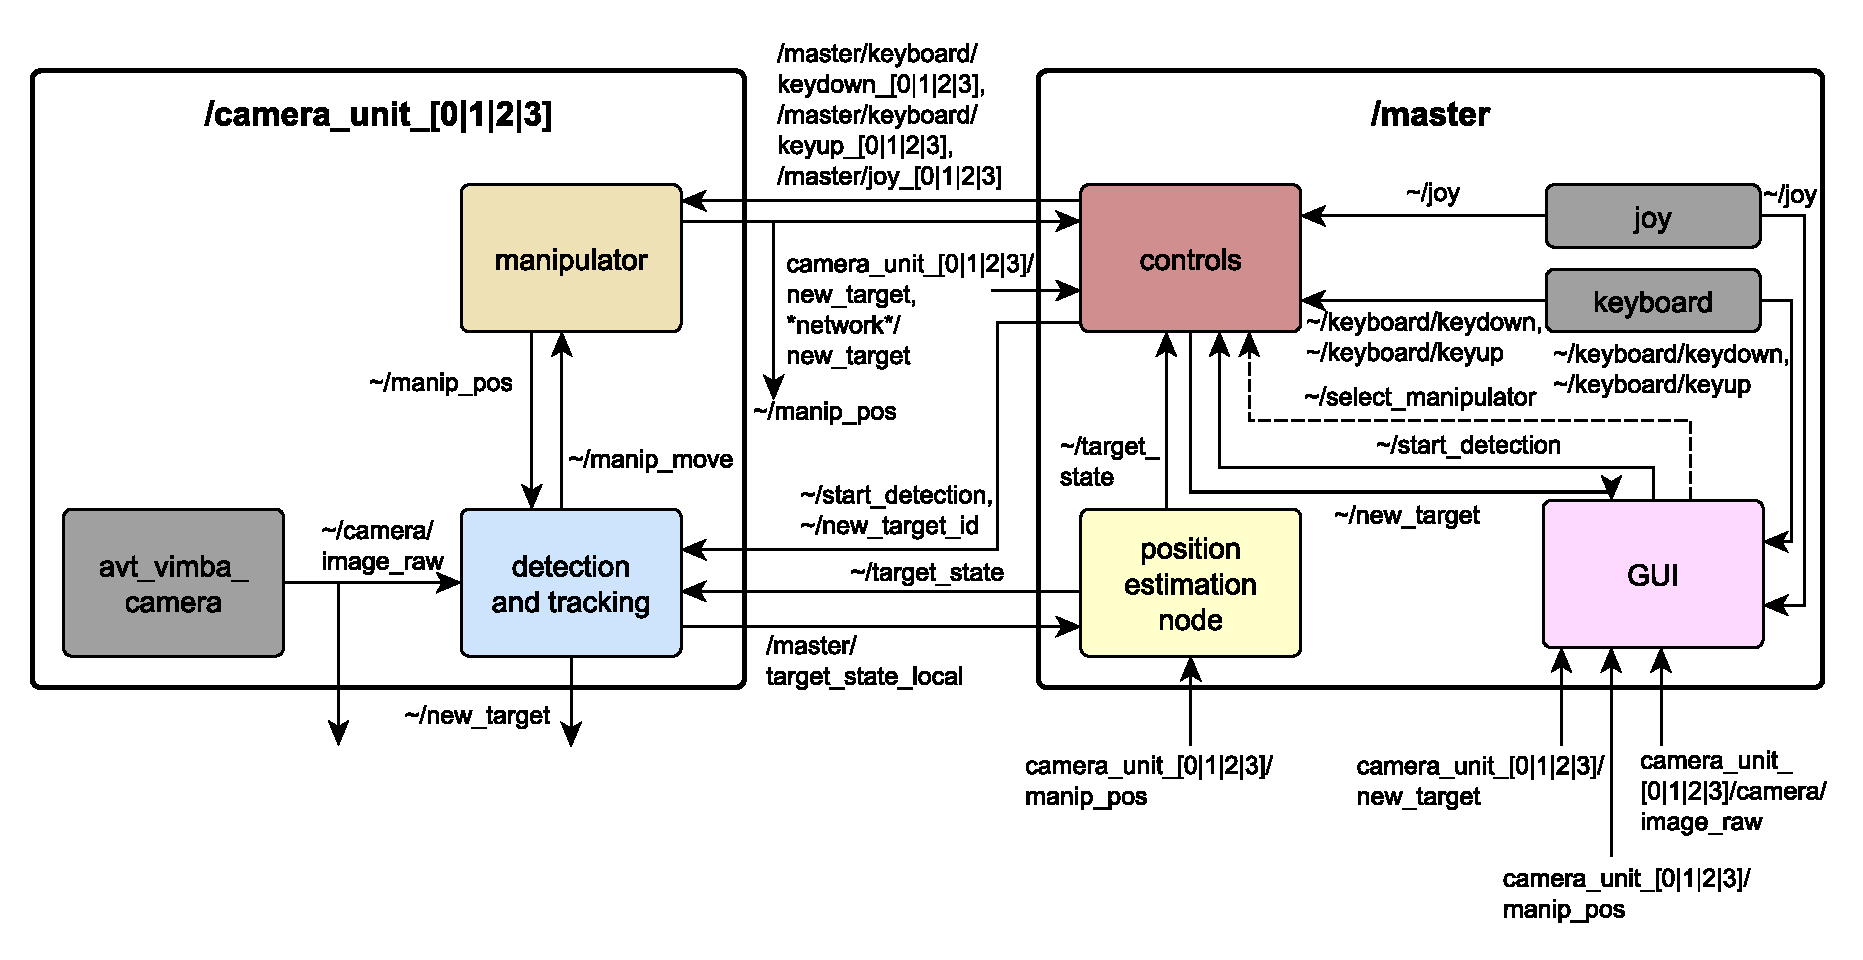
\includegraphics[width=15.5cm]{fig/sw_ols.pdf}
	\caption{The diagram of the software components represented by the ROS nodes. The communication among topics is implemented using ROS topics (normal arrows) and ROS services (dashed arrows).}
	\label{fig:sw_ols}
\end{figure}

The nodes running within the \texttt{master} namespace serve the purpose of the access point for an user (an operator) as well as the main controller of the whole system. The node \texttt{controls} keeps the information about the tracked targets and distributes the workload to the separate camera units based on their position and orientation with regards to the newly discovered target. The node \texttt{position\_estimation} calculates the triangulation and estimates the 3D position of the target. The node \texttt{GUI} implements the graphical user interface allowing the operator to control the system and the nodes \texttt{joy} and \texttt{keyboard} process the events from peripherals.

Each of the namespaces \texttt{camera\_unit\_N} control a separate camera unit. The namespace contains the standard node \texttt{avt\_vimba\_camera} processing the input image stream from Prosilica camera, and implements the node \texttt{manipulator} which controls the manipulator and publishes its state and the node \texttt{detection\_and\_tracking} which performs the computationally most expensive tasks of the object detection, learning its appearance and tracking.

%-------------------------------------------------------------------------
%-------------------------------------------------------------------------
\section{Application of Gazebo} \label{txt:application_of_gazebo}

Gazebo\footnote{The official website of Gazebo: \url{http://gazebosim.org}} is a physical simulator developed by the OSRF\footnote{Open Source Robotic Foundation: \url{http://www.osrfoundation.org/}} providing the tools to model and simulate robots in both indoor and outdoor environment. The simulator has been developed since 2002 and today represents a mature system with wide penetration and support, while being distributed as open source and freeware. 

Since the Gazebo is distributed also as one of the standard packages of the ROS framework it is straightforward to integrate the simulation environment with the already implemented ROS nodes. There are multiple advantages of using the simulator over a development using a real hardware, the main motivations were as follows:

\paragraph{testing a tracker} The Gazebo provides the ROS plugin simulating an RGB camera, which captures the virtual scene and publishes a stream of rendered images. Thus it can be used to test an object tracking algorithm using arbitrarily complex environment and moving objects (see Figure \ref{fig:gazebo_camera_stream}).

%% The screenshot of Gazebo scene and image streams from cameras.
\begin{figure}[htb]
	\centering
	\includegraphics[width=15.5cm]{fig/gazebo_camera_stream.png}
	\caption{The screenshot of a Gazebo simulation (left) consisting of a virtual environment (the gas station), a flying object (the red sphere) and four manipulators. All four virtual camera streams are displayed real-time using \texttt{rviz} tool (right).}
	\label{fig:gazebo_camera_stream}
\end{figure}

\paragraph{testing a manipulator} It is a good practice to include a real hardware in the simulation during the development \cite{on_hw_in_the_loop}. Both actuators and sensors would be difficult to simulate properly, moreover a real manipulator is constrained in terms of the operational range (see Section \ref{txt:camera_unit}), maximum acceleration and speed and communication throughput so it is necessary to thoroughly test its performance. This so called hardware-in-the-loop simulation reveals whether the implementation of motion control is correct and whether the possibilities of the manipulator suffice to track arbitrarily fast (simulated) objects.

\paragraph{testing a triangulation} Thanks to the Gazebo it is possible to simulate a flying object with a-priory set trajectory and evaluate the precision of a position estimation algorithm using comparison between the estimated target position and a ground-truth.

%-------------------------------------------------------------------------
%-------------------------------------------------------------------------
\section{External libraries} \label{txt:external_libraries}

Besides the framework ROS a few other publicly available libraries are used within the implementation.

\paragraph{OpenCV} Open Source Computer Vision Library\footnote{The official website of OpenCV: \url{http://opencv.org}} is a free open source library providing algorithms for image processing, computer vision and machine learning. Version 2.4.11 is used as it is a component of ROS Indigo.

\paragraph{Eigen} This open source C++ template library\footnote{The official website of Eigen: \url{http://eigen.tuxfamily.org}} implements the data structures and methods for fast and convenient solving of linear algebra problems.

\paragraph{OpenTLD} The OpenTLD library\footnote{The official website of OpenTLD: \url{http://www.gnebehay.com/tld}} represents an open source C++ implementation the TLD tracking algorithm (see Section \ref{txt:detection_and_tracking}).	



%=========================================================================
%=========================================================================
\chapter{Experiments and results}
% 1 - 3 ns

- vlastni datova sada
- experimenty na ziskena a porizene datove sade
- === EXPERIMENTY NA REALNYCH DATECH ===

%=========================================================================
%=========================================================================
\chapter{Conclusion}
% 1 - 2 ns

- zhodnocení dosažených výsledků se zvlášť vyznačeným vlastním přínosem studenta
- zhodnocení z pohledu dalšího vývoje projektu vzhledem k diplomové práci
- moznosti dalsiho vyvoje: modelovani okoli ve 3D nebo vyuziti teto info z mapy, paralelizace narocnych casti na GPU
- veci, co se zatim nebraly v uvahu
	- system je umisten na rozhrani dvou a vice UTM zon


